\documentclass{article}\usepackage[]{graphicx}\usepackage[]{color}
%% maxwidth is the original width if it is less than linewidth
%% otherwise use linewidth (to make sure the graphics do not exceed the margin)
\makeatletter
\def\maxwidth{ %
  \ifdim\Gin@nat@width>\linewidth
    \linewidth
  \else
    \Gin@nat@width
  \fi
}
\makeatother

\definecolor{fgcolor}{rgb}{0.345, 0.345, 0.345}
\newcommand{\hlnum}[1]{\textcolor[rgb]{0.686,0.059,0.569}{#1}}%
\newcommand{\hlstr}[1]{\textcolor[rgb]{0.192,0.494,0.8}{#1}}%
\newcommand{\hlcom}[1]{\textcolor[rgb]{0.678,0.584,0.686}{\textit{#1}}}%
\newcommand{\hlopt}[1]{\textcolor[rgb]{0,0,0}{#1}}%
\newcommand{\hlstd}[1]{\textcolor[rgb]{0.345,0.345,0.345}{#1}}%
\newcommand{\hlkwa}[1]{\textcolor[rgb]{0.161,0.373,0.58}{\textbf{#1}}}%
\newcommand{\hlkwb}[1]{\textcolor[rgb]{0.69,0.353,0.396}{#1}}%
\newcommand{\hlkwc}[1]{\textcolor[rgb]{0.333,0.667,0.333}{#1}}%
\newcommand{\hlkwd}[1]{\textcolor[rgb]{0.737,0.353,0.396}{\textbf{#1}}}%

\usepackage{framed}
\makeatletter
\newenvironment{kframe}{%
 \def\at@end@of@kframe{}%
 \ifinner\ifhmode%
  \def\at@end@of@kframe{\end{minipage}}%
  \begin{minipage}{\columnwidth}%
 \fi\fi%
 \def\FrameCommand##1{\hskip\@totalleftmargin \hskip-\fboxsep
 \colorbox{shadecolor}{##1}\hskip-\fboxsep
     % There is no \\@totalrightmargin, so:
     \hskip-\linewidth \hskip-\@totalleftmargin \hskip\columnwidth}%
 \MakeFramed {\advance\hsize-\width
   \@totalleftmargin\z@ \linewidth\hsize
   \@setminipage}}%
 {\par\unskip\endMakeFramed%
 \at@end@of@kframe}
\makeatother

\definecolor{shadecolor}{rgb}{.97, .97, .97}
\definecolor{messagecolor}{rgb}{0, 0, 0}
\definecolor{warningcolor}{rgb}{1, 0, 1}
\definecolor{errorcolor}{rgb}{1, 0, 0}
\newenvironment{knitrout}{}{} % an empty environment to be redefined in TeX

\usepackage{alltt}

%%%%%%%%%%%%%%%%
% Header for attribution
%%%%%%%%%%%%%%%%

%\pagestyle{fancy}
%
%\fancyhead{}
%
%\renewcommand{\headrulewidth}{0.25pt}
%\renewcommand{\footrulewidth}{0pt}
%\headsep = 30pt 
%\footskip = 30pt
%
%\chead{{\footnotesize Derivative of \href{http://www.opeintro.org}{\textit{OpenIntro}} project}}

%%%%%%%%%%%%%%%%
% Packages
%%%%%%%%%%%%%%%%

\usepackage[sc]{mathpazo}
%\usepackage[T1]{fontenc}
\usepackage{geometry}
\geometry{verbose,tmargin=2cm,bmargin=2.2cm,lmargin=2.5cm,rmargin=2.5cm}
\setcounter{secnumdepth}{2}
\setcounter{tocdepth}{2}
\usepackage{url}
\usepackage{xcolor}
\usepackage[parfill]{parskip}
\usepackage{graphicx}
\usepackage{amssymb}
\usepackage{amsmath}
\usepackage{epstopdf}
\usepackage{enumerate}
\usepackage{colortbl}
\usepackage{xcolor}
\usepackage{sectsty}
\usepackage{multicol}
\usepackage{fancyhdr}
\usepackage{changepage}
\usepackage{textcomp}
\usepackage{endnotes}
\usepackage{breakurl}

%%%%%%%%%%%%%%%%
% Colors and hyperref
%%%%%%%%%%%%%%%%

\definecolor{oiB}{rgb}{.337,.608,.741}
\definecolor{oiR}{rgb}{.941,.318,.200}
\definecolor{oiG}{rgb}{.298,.447,.114}
\definecolor{oiY}{rgb}{.957,.863,0}

\usepackage[unicode=true, pdfusetitle, bookmarks=true, bookmarksnumbered=true, bookmarksopen=true, bookmarksopenlevel=2, breaklinks=false, pdfborder={0 0 1}, backref=false, colorlinks=true, linkcolor = oiB, urlcolor= oiB]{hyperref}
\hypersetup{pdfstartview={XYZ null null 1}}

%%%%%%%%%%%%%%%%%
%% Color section headings
%%%%%%%%%%%%%%%%%

\allsectionsfont{\color{oiB}}              
 
%%%%%%%%%%%%%%%%
% Exercise environment
%%%%%%%%%%%%%%%%

\newenvironment{exercise}
{
\addvspace{5mm}
\begin{adjustwidth}{0em}{3em}
\begin{itemize}\item[]\refstepcounter{equation}\noindent\normalsize\textbf{\textcolor{oiB}{Exercise \theexercise}}
}
{\normalsize

\addvspace{3mm}
\end{itemize}
\end{adjustwidth}
}

\newcommand\theexercise{\arabic{equation}}

%%%%%%%%%%%%%%%%
% Menu items
%%%%%%%%%%%%%%%%

\newcommand{\menu}[1]{\textsf{#1}}

%%%%%%%%%%%%%%%%
% Formatted url
%%%%%%%%%%%%%%%%

\newcommand{\web}[1]{\urlstyle{same}\textit{\url{#1}}}

%%%%%%%%%%%%%%%%
% Footnote using symbols
% 1 - *
% 2 - dagger
% 3 - double dagger
% 4 - ... 9 (see page 175 of the latex manual)
% http://help-csli.stanford.edu/tex/latex-footnotes.shtml
%%%%%%%%%%%%%%%%

\long\def\symbolfootnote[#1]#2{\begingroup%
\def\thefootnote{\fnsymbol{footnote}}\footnote[#1]{#2}\endgroup}

%%%%%%%%%%%%%%%%
% Non-numbered footnote for license and attribution
%%%%%%%%%%%%%%%%

\newcommand{\license}[1]{\let\thefootnote\relax\footnotetext{#1}}

%%%%%%%%%%%%%%%%
% Set padding in code chunk boxes
%%%%%%%%%%%%%%%%

\setlength\fboxsep{2mm}

%%%%%%%%%%%%%%%%
% Place spacing between text and code chunk boxes
%%%%%%%%%%%%%%%%

\ifdefined\knitrout
  \renewenvironment{knitrout}{
    \vspace{1em}
  }{
    \vspace{1em}
  }
\else
\fi

%%%%%%%%%%%%%%%%
% Redefine inline code commands to change the font to texttt
%%%%%%%%%%%%%%%%

\renewcommand{\hlfunctioncall}[1]{\textcolor[rgb]{0.11,0.53,0.93}{\texttt{#1}}}%

\renewcommand{\hlstring}[1]{\textcolor[rgb]{0.65,0.50,0.39}{\texttt{#1}}}%

\renewcommand{\hlsymbol}[1]{\textcolor[rgb]{0.387,0.581,0.148}{\texttt{#1}}}%

\renewcommand{\hlkeyword}[1]{\textcolor[rgb]{0.31,0.65,0.76}{\texttt{#1}}}%

\renewcommand{\hlargument}[1]{\textcolor[rgb]{0.31,0.41,0.53}{\texttt{#1}}}%

\renewcommand{\hlnumber}[1]{\textcolor[rgb]{0.387,0.581,0.148}{\texttt{#1}}}%


\IfFileExists{upquote.sty}{\usepackage{upquote}}{}

\begin{document}

\license{This is a product of OpenIntro that is released under a Creative Commons Attribution-ShareAlike 3.0 Unported (\web{http://creativecommons.org/licenses/by-sa/3.0}). This lab was written by Andrew Bray and Mine \c{C}etinkaya-Rundel.}


\section*{Lab 6B: Testing for Goodness of Fit}

\subsection*{2009 Iran Election}
On June 12 2009, the Republic of Iran \href{http://en.wikipedia.org/wiki/Iranian_presidential_election,_2009}{held an election} where President Mahmoud Ahmadinejad sought re-election against three challengers.  When it was announced that Ahmadinejad had won with 62\% of the vote, there were widespread allegations of election fraud.

There are many methods, both quantitative and qualitative, to detect election fraud.  In this lab we will explore just one proposed method.

\subsection*{The Data}
The election commission released total vote counts for each candidate by region.  Let's load up this data.\footnote{}

\begin{knitrout}
\definecolor{shadecolor}{rgb}{0.969, 0.969, 0.969}\color{fgcolor}\begin{kframe}
\begin{alltt}
\hlstd{get_digit} \hlkwb{<-} \hlkwa{function}\hlstd{(}\hlkwc{x}\hlstd{,} \hlkwc{which_digit} \hlstd{=} \hlstr{"first"}\hlstd{) \{}
    \hlkwa{if} \hlstd{(}\hlkwd{is.na}\hlstd{(}\hlkwd{match}\hlstd{(which_digit,} \hlkwd{c}\hlstd{(}\hlstr{"first"}\hlstd{,} \hlstr{"last"}\hlstd{)))) \{}
        \hlkwd{stop}\hlstd{(}\hlstr{"which_digit must be first or last"}\hlstd{)}
    \hlstd{\}}
    \hlkwa{if} \hlstd{(which_digit} \hlopt{==} \hlstr{"first"}\hlstd{) \{}
        \hlkwd{as.integer}\hlstd{(}\hlkwd{head}\hlstd{(}\hlkwd{strsplit}\hlstd{(}\hlkwd{as.character}\hlstd{(x),} \hlstr{""}\hlstd{)[[}\hlnum{1}\hlstd{]],} \hlkwc{n} \hlstd{=} \hlnum{1}\hlstd{))}
    \hlstd{\}} \hlkwa{else} \hlstd{\{}
        \hlkwd{as.integer}\hlstd{(}\hlkwd{tail}\hlstd{(}\hlkwd{strsplit}\hlstd{(}\hlkwd{as.character}\hlstd{(x),} \hlstr{""}\hlstd{)[[}\hlnum{1}\hlstd{]],} \hlkwc{n} \hlstd{=} \hlnum{1}\hlstd{))}
    \hlstd{\}}
\hlstd{\}}
\hlcom{# read in iran data}
\hlstd{iran} \hlkwb{<-} \hlkwd{read.csv}\hlstd{(}\hlstr{"iran.csv"}\hlstd{,} \hlkwc{header} \hlstd{=} \hlnum{TRUE}\hlstd{)}
\hlstd{digits_iran} \hlkwb{<-} \hlkwd{sapply}\hlstd{(iran}\hlopt{$}\hlstd{total_votes_cast,} \hlkwc{FUN} \hlstd{= get_digit)}
\hlstd{obs} \hlkwb{<-} \hlkwd{table}\hlstd{(digits_iran)}
\hlkwd{barplot}\hlstd{(obs)}
\end{alltt}
\end{kframe}
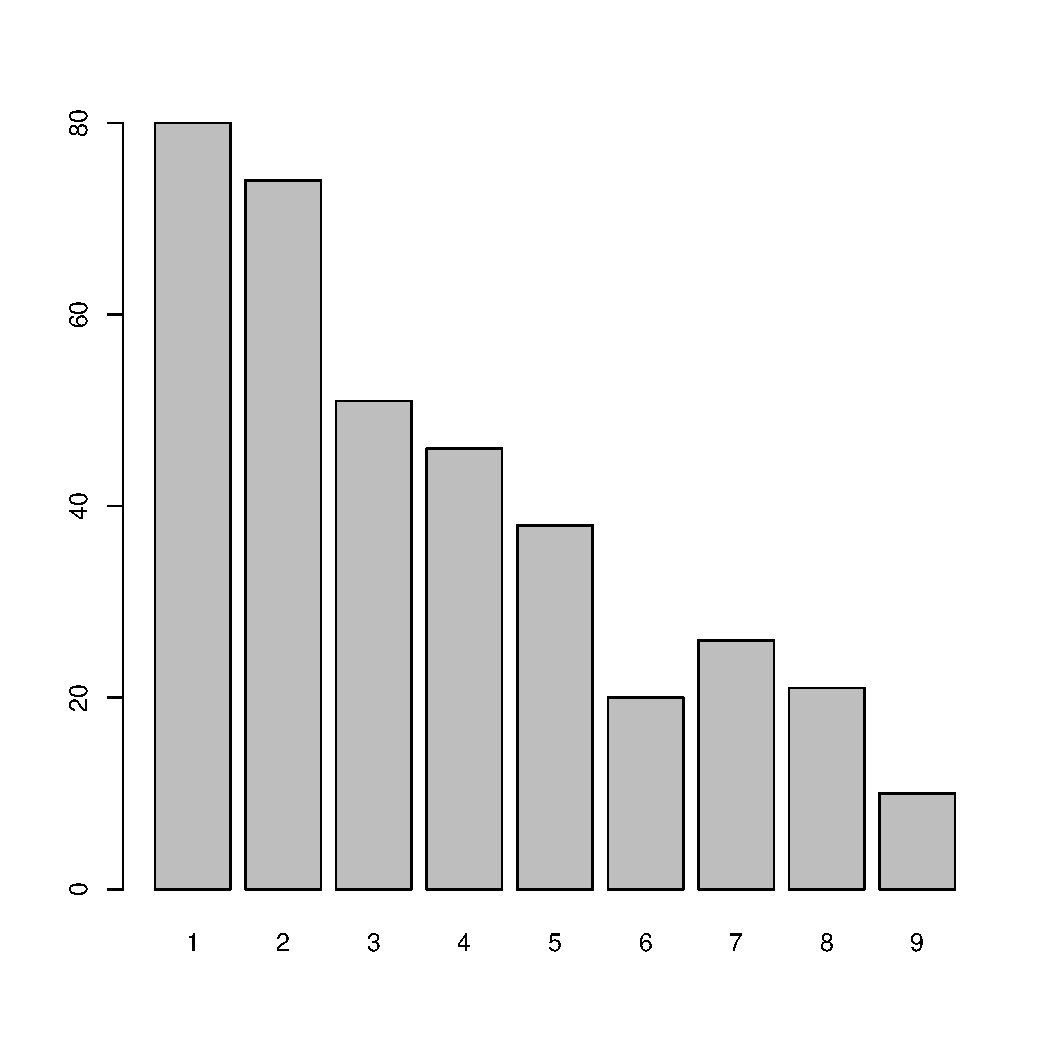
\includegraphics[width=\maxwidth]{figure/load-iran-data1} 
\begin{kframe}\begin{alltt}
\hlcom{# compare to Benfords dist}
\hlstd{n} \hlkwb{<-} \hlkwd{dim}\hlstd{(iran)[}\hlnum{1}\hlstd{]}
\hlstd{benfords_p} \hlkwb{<-} \hlkwd{log10}\hlstd{(}\hlnum{1} \hlopt{+} \hlnum{1}\hlopt{/}\hlnum{1}\hlopt{:}\hlnum{9}\hlstd{)}
\hlstd{expected} \hlkwb{<-} \hlstd{benfords_p} \hlopt{*} \hlstd{n}
\hlstd{chistat} \hlkwb{<-} \hlkwd{sum}\hlstd{(((obs} \hlopt{-} \hlstd{expected)}\hlopt{^}\hlnum{2}\hlstd{)}\hlopt{/}\hlstd{expected)}
\hlkwd{pchisq}\hlstd{(chistat,} \hlkwc{df} \hlstd{=} \hlnum{8}\hlstd{,} \hlkwc{lower.tail} \hlstd{=} \hlnum{FALSE}\hlstd{)}
\end{alltt}
\begin{verbatim}
## [1] 0.006836
\end{verbatim}
\begin{alltt}
\hlcom{# read in norway data}
\hlstd{norway} \hlkwb{<-} \hlkwd{read.csv}\hlstd{(}\hlstr{"norway.csv"}\hlstd{,} \hlkwc{header} \hlstd{=} \hlnum{TRUE}\hlstd{)}
\hlstd{digits_norway} \hlkwb{<-} \hlkwd{sapply}\hlstd{(norway}\hlopt{$}\hlstd{total_votes_cast,} \hlkwc{FUN} \hlstd{= get_digit)}
\hlstd{obs} \hlkwb{<-} \hlkwd{table}\hlstd{(digits_norway)}
\hlkwd{barplot}\hlstd{(obs)}
\end{alltt}
\end{kframe}
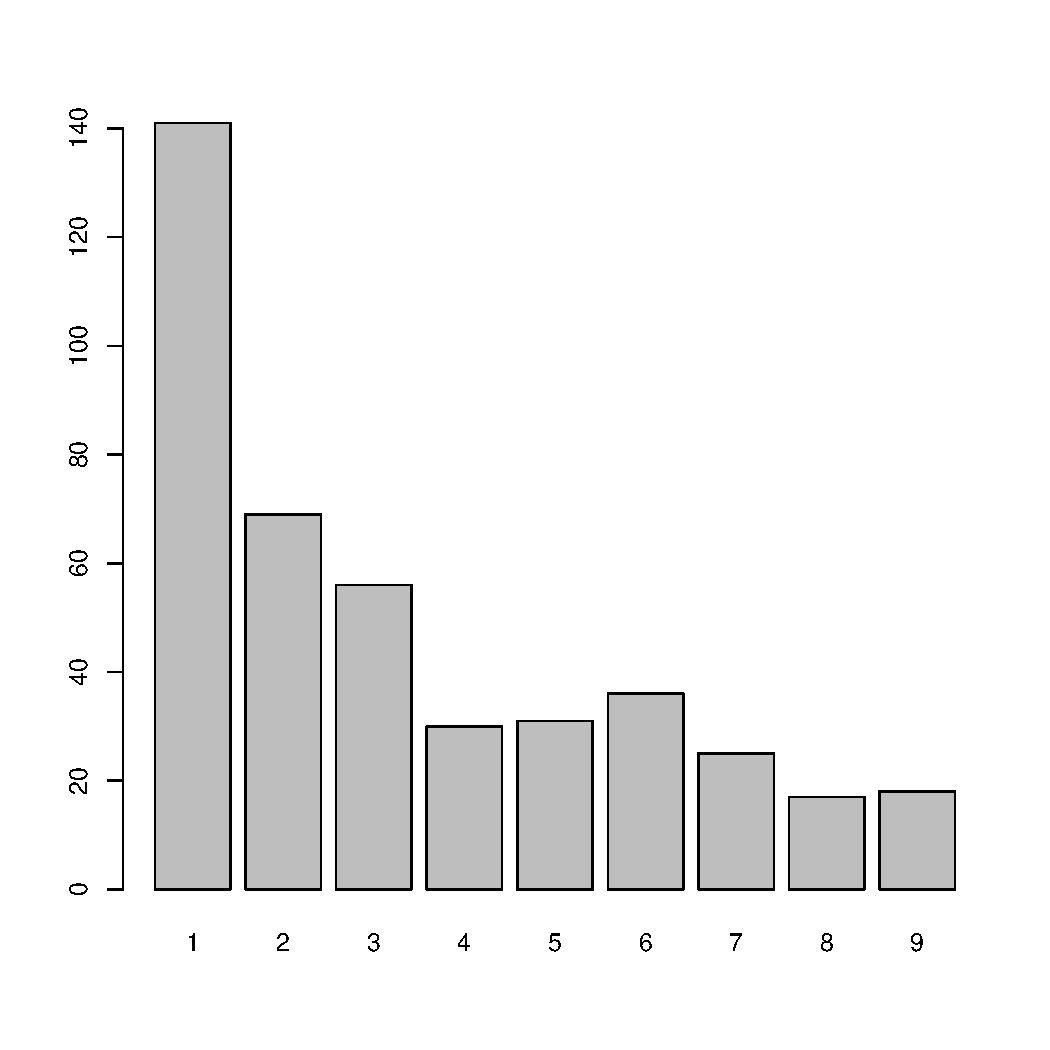
\includegraphics[width=\maxwidth]{figure/load-iran-data2} 
\begin{kframe}\begin{alltt}
\hlcom{# compare to Benfords dist}
\hlstd{n} \hlkwb{<-} \hlkwd{dim}\hlstd{(norway)[}\hlnum{1}\hlstd{]}
\hlstd{expected} \hlkwb{<-} \hlstd{benfords_p} \hlopt{*} \hlstd{n}
\hlstd{chistat} \hlkwb{<-} \hlkwd{sum}\hlstd{(((obs} \hlopt{-} \hlstd{expected)}\hlopt{^}\hlnum{2}\hlstd{)}\hlopt{/}\hlstd{expected)}
\hlkwd{pchisq}\hlstd{(chistat,} \hlkwc{df} \hlstd{=} \hlnum{8}\hlstd{,} \hlkwc{lower.tail} \hlstd{=} \hlnum{FALSE}\hlstd{)}
\end{alltt}
\begin{verbatim}
## [1] 0.3979
\end{verbatim}
\end{kframe}
\end{knitrout}


David: do these calculations look right?  I haven't worked with this data for awhile, but for some reason I remember that the iran data didn't mesh with benfords, suggesting fraud but then the norway data didn't either, suggesting . . . that the assumptions of benfords don't really hold in vote total settings.  Running, it here, though, the Norwegian data looks fine by Benfords.  I guess I could try getting county level data from the US and trying there...


\end{document}
